\chapter*{Задача с тележкой}

\section*{Интерпретация исходной задачи}

\begin{figure}[h!]
    \centering
    \begin{minipage}{.6\textwidth}
        \centering
        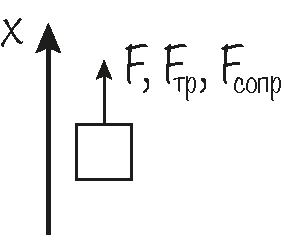
\includegraphics[height=.3\linewidth]{pic_3_1.pdf}
    \end{minipage}%
    \begin{minipage}{.4\textwidth}
        % \centering
        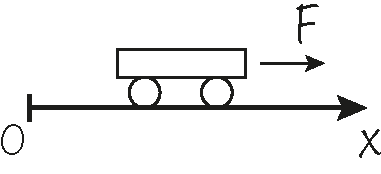
\includegraphics[height=.35\linewidth]{pic_3_2.pdf}
    \end{minipage}
\end{figure}

\textit{Движению тележки (или, например, лифта), вызванному тягой двигателя $F_{\text{вн}}$, будут препятствовать вязкое трение $F_{\text{тр}} = -k \dot{x}$ и сопротивление среды $F_{\text{сопр}} = -d\dot{x}^2$}:
$$
    m \ddot{x} = -k\dot{x} - d \dot{x}^2 + F_{\text{вн}}
$$
$$
    \Downarrow
$$
$$
    \ddot{x} = -\frac{k}{m} \dot{x} - \frac{d}{m} \dot{x}^2 + \frac{F_{\text{вн}}}{m}.
$$
\textit{Обозначая $\frac{k}{m} = u_1 \in [u_1^{min}, u_1^{max}]$, $\frac{d}{m} = u_2 \in [u_2^{min}, u_2^{max}]$, $\frac{F_{\text{вн}}}{m} = u_3 \in [0, u_3^{max}]$, и приводя к нормальному виду:}
$$
    x_1 = x, \; x_2 = \dot{x},
$$
получим систему следующего вида:
$$
    \begin{aligned}
        & \left\{
            \begin{aligned}
                & \dot{x}_1 = x_2, \\
                & \dot{x}_2 = - (u_1x_2 + u_2 x_2^2) + u_3,
            \end{aligned}
        \right.\\
        & u_1 \in [u_1^{min}, u_1^{max}], & 0 < u_1^{min} < u_1^{max}, \\
        & u_2 \in [u_2^{min}, u_2^{max}], & 0 < u_2^{min} < u_2^{max}, \\
        & u_3 \in [0, u_3^{max}],         & 0 < u_3^{max}.
    \end{aligned}
$$

Добавляем начальные условия, завершая формулировку задачи:
$$
\begin{aligned}
    & t_0 = 0, \\
    & x_1 (0) = x_2 (0) = 0, \\
    & t_1 = T > 0 \text{ --- фикс. момент времени}, \\
    & x_1(t) = L, \\
    & x_2(t) = \varepsilon > 0.
\end{aligned}
$$
При этом предполагается, что $L > T \varepsilon$, то есть для попадания в конечную точку нельзя ехать с некоторой минимальной тягой, необходимо именно разогнаться, после чего остановиться.

Оптимальность искомого управления будет определяться функционалом
$$
J = \int\limits_{0}^{T} u_3(t) dt \to \inf\limits_{u(\cdot)}.
$$

Таким образом, задача состоит в перемещении тележки на прямой из точки с координатой $0$ в точку с координатой $L$ с остановкой в конечный момент времени при минимизации усилий, прилагаемых для этого перемещения.

\begin{remark}
    Почему на правом конце не используется простое условие $x_2(T) = 0$? Поскольку интерпретация задачи предполагает остановку в конечный момент времени, $u_3(T) = 0$. Добавляя к этому нулевое значение на правом конце и интегрируя уравнение на $x_2$ в обратном времени, получим нулевое решение ОДУ $x_2 \equiv 0$, которое, очевидно, не даёт решение исходной задачи.
\end{remark}

Итак, обобщим всё сказанное.

\section*{Постановка задачи}
$$
    \left\{
            \begin{aligned}
                & \dot{x}_1 = x_2, \\
                & \dot{x}_2 = - (u_1x_2 + u_2 x_2^2) + u_3,
            \end{aligned}
        \right.
$$
$$
    \begin{aligned}
        & u_1 \in [u_1^{min}, u_1^{max}], & 0 < u_1^{min} < u_1^{max}, \\
        & u_2 \in [u_2^{min}, u_2^{max}], & 0 < u_2^{min} < u_2^{max}, \\
        & u_3 \in [0, u_3^{max}],         & 0 < u_3^{max}, \\
    \end{aligned}
$$
$$
    \begin{aligned}
        & t_0 = 0, \; x_1 (0) = x_2 (0) = 0, \\
        & t_1 = T > 0, \; x_1(t) = L, x_2(t) = \varepsilon > 0, \; L > T \varepsilon,
    \end{aligned}
$$
$$
J = \int\limits_{0}^{T} u_3(t) dt \to \inf\limits_{u(\cdot)}.
$$

\section*{Шаг 1. ПМП}
Выпишем ПМП для рассматриваемой задачи (автономная система, задача точка-точка с фиксированным $t_1$).

Вносим функционал качества в исходную систему:
$$
    \left\{
        \begin{aligned}
            & \dot{x}_0 = u_3, \\
            & \dot{x}_1 = x_2, \\
            & \dot{x}_2 = - (u_1 x_2 + u_2 x_2^2) + u_3.
        \end{aligned}
    \right.
$$
Выписываем функцию Гамильтона-Понтрягина:
$$
    \tilde{\mathscr{H}} = \psi_0 u_3 + \psi_1 x_2 + \psi_2 (u_3 - u_1 x_2 - u_2x_2^2).
$$

\textbf{Тогда ПМП принимает следующий вид:}

Пусть $\{x^*(\cdot), u^*(\cdot)\}$ --- оптимальная пара (при $t_1 = t_1^*, t \in [t_0^*, t_1^*], t_0 = t_0^*$).

Тогда $\exists \tilde{\psi}^* \colon [t_0^*, t_1^*] \to \R^{n+1}$ такая, что:
\begin{enumerate}
    \item[(УН) 1)] $\psi^*(t) \neq 0, t \in [0, T]$,
    \item[(СС) 2)] 
    $$
        \left\{
            \begin{aligned}
                & \dot{\psi^*}_0 = -\frac{\d \tilde{\mathscr{H}}}{\d x_0} = 0, \\
                & \dot{\psi^*}_1 = -\frac{\d \tilde{\mathscr{H}}}{\d x_1} = 0, \\
                & \dot{\psi^*}_2 = -\frac{\d \tilde{\mathscr{H}}}{\d x_2} = -\psi_1^{0,*} + \psi_2^* (u_1^* + 2 u_2^* x_2^*).
            \end{aligned}
        \right.
    $$
    \item[(УМ) 3)] $\tilde{\mathscr{H}}(\tilde{\psi}^*(t), \tilde{x}^*(t), u^*(t)) = \sup\limits_{u} \tilde{\mathscr{H}}(\tilde{\psi}^*(t), \tilde{x}^*(t), u)$ для п.в. $t \in [0, T]$.
    \item[4)] $\psi_0^* (\cdot) \equiv const \leqslant 0$, \\
            $\tilde{\mathscr{M}}(\tilde{\psi}^*(t), \tilde{x}^*(t)) \equiv const = 0$.
\end{enumerate}

Второе условие из 4) использовать при решении задачи будет неудобно, поэтому использовать его мы не будем.

Из условия максимума получаем (далее опускаем обозначения звёздочек для лаконичности всюду, кроме $u^*$):
\begin{enumerate}
    \item[$u_1$:] $-\psi_2 x_2 u_1 \to \max \thus u_1^* = \left\{ \begin{aligned}
        & u_1^{min}, &\psi_2 x_2 > 0, \\
        & [u_1^{min}, u_1^{max}], &\psi_2 x_2 = 0, \\
        & u_1^{max}, &\psi_2 x_2 < 0,
    \end{aligned} \right. $
    \item[$u_2$:] $-\psi_2 x_2^2 u_2 \to \max \thus u_2^* = \left\{ \begin{aligned}
        & u_2^{min}, &\psi_2 > 0, x_2 \neq 0, \\
        & [u_2^{min}, u_2^{max}], &\psi_2 x_2 = 0, \\
        & u_2^{max}, &\psi_2 < 0, x_2 \neq 0,
    \end{aligned} \right. $
    \item[$u_3$:] $-\psi_2 x_2^2 u_2 \to \max \thus u_3^* = \left\{ \begin{aligned}
        & u_3^{max}, &\psi_0^0 + \psi_2 > 0, \\
        & [0, u_3^{max}], &\psi_0^0 + \psi_2 = 0, \\
        & 0, &\psi_0^0 + \psi_2 < 0.
    \end{aligned} \right. $
\end{enumerate}
При этом при некоторых значениях $(\psi, x)$ значения компонент управления $u_i$ невозможно определить однозначно.

\begin{define}
    \textbf{Особым режимом} называется состояние системы, в котором оптимальное управление однозначно не выражается через $(\psi, x)$ в течение отрезка времени положительной длины.
\end{define}

\section*{Шаг 2. Нормальный случай}
Пусть $\psi_0 \equiv \psi_0^0 < 0$, тогда БОО положим $\psi_0 = -1$. Тогда из (УМ):
$$
    u_3^* = \left\{ \begin{aligned}
        & u_3^{max}, &\psi_2 > 1, \\
        & [0, u_3^{max}], &\psi_2 = 1, \\
        & 0, &\psi_2 < 1.
    \end{aligned} \right.
$$

Обозначим $\psi_1(0) = \psi_1^0$, $\psi_2(0) = \psi_2^0$ и исследуем поведение системы при различных значениях этих параметров.

\section*{Шаг 2.1. Движение при $\psi_2^0 > 1$}
\section*{2.1.1 Движение в окрестности нуля}
Пусть $\psi_2^0 > 1$, тогда в некоторой окрестности $[0, \tau]$ нуля будет выполняться $u_3^* = u_3^{max}$ \textit{(найдётся такая окрестность, в которой функция $\psi_2$ будет непрерывна, следовательно, и уравнение будет выражаться соответствующим образом)}. Тогда в этой окрестности
$$
    \dot{x}_2 = u_3^{max} - (u_1 + u_2 x_2) x_2.
$$
В этой окрестности (достаточно малой) $x_2 \approx 0$, $u_3^{max} > 0$, то есть $\dot{x}_2 > 0$.

\textit{С точки зрения интерпретации условия $x_2(0) = 0$, $\dot{x_2}(0+) > 0$ означают, что в начале движения будет происходить ускорение}.

Таким образом, в этом случае существует такое $\tau > 0$, что:
$$
\begin{aligned}
    & \forall t \in (o, \tau] \thus \psi_2(t) > 1, \\
    & \forall t \in (o, \tau] \thus x_2(t) > 0, \\
    & \forall t \in (o, \tau] \thus \left\{ \begin{aligned} & u_1^* = u_1^{min}, \\ & u_2^* = u_2^{min}. \end{aligned} \right.
\end{aligned}
$$

Тогда на отрезке $[0, \tau]$ динамика системы описывается следующей системой дифференциальных уравнений:
$$
    \left\{
    \begin{aligned}
        & \dot{x}_1 = x_2, \\
        & \dot{x}_2 = u_3^{max} - (u_1^{min} + u_2^{min} x_2) x_2, \\
        & \dot{\psi}_1 = 0, \\
        & \dot{\psi}_2 = - \psi_1 + \psi_2 (u_1^{min} + 2 u_2^{min} x_2), \\
    \end{aligned}
    \right.
$$
с начальным условиями
$$
    \left\{
    \begin{aligned}
        & \dot{x}_2(0) = 0, \\
        & \dot{\psi}_2(0) = \psi_2^0 > 1. \\
    \end{aligned}
    \right.
$$
В этой системе нас будут интересовать второе и четвёртое уравнение, поскольку только значения $x_2$ и $\psi_2$ влияют на выбранное управление, соответственно, могут привести к переключению. До тех пор, пока переключение не произошло, движение описываться указанной системой. \textit{Понимая это, начальные условия на $x_1$ и $\psi_1$ мы сразу опустили}.

Движение системы описывается указанной системой дифференциальных уравнений до тех пор, пока $\psi_2 > 1$ и $x_2 > 0$. Исследуем, каким образом будут вести себя траектории системы 
$$
    \left\{
    \begin{aligned}
        & \dot{x}_2 = u_3^{max} - (u_1^{min} + u_2^{min} x_2) x_2, \\
        & \dot{\psi}_2 = - \psi_1 + \psi_2 (u_1^{min} + 2 u_2^{min} x_2). \\
    \end{aligned}
    \right.
$$

Схематично изобразим их на рисунке:

\begin{figure}[H]
    \centering
    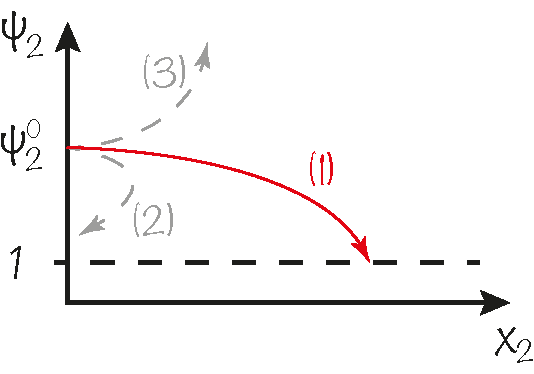
\includegraphics[height=.3\linewidth]{pic_3_3.pdf}
\end{figure}

\subsection*{Траектория (2)}
Покажем, что такое невозможно. Найдём особые точки для $x_2$:
$$
\dot{x}_2 = 0 \Leftrightarrow u_2^{min} x_2^2 + u_1^{min} x_2 - u_3^{max} = 0.
$$
Разрешая последнее квадратное уравнение относительно $x_2$, получим положительный дискриминант:
$$
D = \left(u_1^{min}\right)^2 + 4 u_2^{min} u_3^{max} > 0
$$
и два корня (разных знаков):
$$
    x_2 = \frac{- u_1^{min} \pm \sqrt{D}}{2 u_2^{min}}.
$$

\begin{figure}[H]
    \centering
    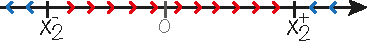
\includegraphics[width=.4\linewidth]{pic_3_11.pdf}
\end{figure}

Таким образом, в точке $x_2^+$ находится аттрактор, к которому будут стремиться траектории системы, и в обратную сторону (на уменьшение $x_2$) они направлены не будут. Случай траектории (2) невозможен.

При этом мы сразу отсекаем случай ненарисованной четвёртой траектории, отвечающей условиям $\psi_2 \uparrow$, $x_2 \downarrow$.

\subsection*{Траектория (3)}
Покажем, что такая траектория движения не приведёт нас к решению задачи. Действительно, в предположении $\dot{\psi_2} > 0$ из уравнения
$$
\dot{\psi}_2 = -\psi_1^0 + \psi_2 u_1^{min}
$$
получаем, что такое поведение возможно в случае, когда
$$
\psi_1^0 < \psi_2 u_1^{min}.
$$
Поскольку $\psi_2$ по нашему предположению возрастает, то условие будет выполнено всегда, если $\psi_1^0 < \psi_2^0 u_1^{min}$. Тогда $\tau = +\infty$, а $x_2$ и $\psi_2$ бесконечно возрастают (рост $x_2$ показан для траектории (2)). Тогда условие $x_2(T) = \varepsilon$ не может быть выполнено (в предположении, что $\varepsilon$ достаточно маленькое).

Таким образом, указанная траектория не даёт решения исходной задачи.

\subsection*{Траектория (1)}
Таким образом, имеет смысл рассматривать только те пары $(\psi_1^0, \psi_2^0)$, для которых $\exists \tau_I \in (o, \tau)$: $\psi_2(\tau_I) = 1$, то есть имеет место переключение.

\section*{2.1.2 Перепараметризация}
Проинтегрировав систему и разрешив уравнение
$$
    \psi_2(t) = 1
$$
относительно $t$, найдём момент первого переключения $\tau_I$. При этом в силу свойств решения дифференциального уравнения зависимость $\tau_I(\psi_1^0, \psi_2^0)$ будет достаточно гладкой. Пользуясь этим, уйдём от рассмотрения параметра $\psi_2^0$ в пользу $\tau_I$:
$$
(\psi_1^0, \psi_2^0) \rightarrow (\psi_1^0, \tau_I).
$$
В случае необходимости, значение $\psi_2 = \psi_2^0(\psi_1^0, \tau_I)$ может быть найдено за счёт интегрирования рассматриваемой системы для движения на $[0, \tau]$ в обратном времени.

Перебирать параметр $\tau_I \in [0, T]$ проще, чем всевозможные значения изначального $\psi_2 \in \R$. \textbf{При этом важно, что мы показали невозможность остальных случаев! Если бы какой-то альтернативных вариантов движения по траекториям (2) или (3) был бы возможен, их требовалось бы рассмотреть отдельно. В противном случае при осуществлённой замене параметров потерялась бы часть возможных решений, среди которых может быть \textit{оптимальное}}.

Зададимся теперь вопросом, что будет происходить при $t > \tau_I$. Поскольку ранее показано $x_2 \uparrow$, управления на следующем участке пути примут следующий вид ($u_3$ пока не определено, остальные остаются такими же, какими были):

$$
    \left\{
    \begin{aligned}
        & \dot{x}_2 = u_3 - (u_1^{min} + u_2^{min} x_2) x_2, \\
        & \dot{\psi}_2 = - \psi_1 + \psi_2 (u_1^{min} + 2 u_2^{min} x_2). \\
    \end{aligned}
    \right.
$$

Возвращаясь к виду оптимального управления $u_3^*$:
$$
    u_3^* = \left\{ \begin{aligned}
        & u_3^{max}, &\psi_2 > 1, \\
        & [0, u_3^{max}], &\psi_2 = 1, \\
        & 0, &\psi_2 < 1.
    \end{aligned} \right.
$$
приходим к выводу, что возможны два варианта: простое переключение в $u_3^* = 0$ и особый режим. Начнём именно со второго случая, после чего сведём к нему первый.

\section*{2.1.3 Особый режим при переходе через $\tau_I$}
Для того, чтобы система находилась в особом режиме (по компоненте управления $u_3$), необходимо, чтобы при $t \in [\tau_I, \tau_I + \delta)$ выполнялось $\psi_2(t) = 1$. В каком случае это возможно? Из последнего уравнения следует, что на этом интервале
\begin{equation}\label{eq:nonlin_3_1}
    \dot{\psi}_2(t) = 0 \thus -\psi_1^0 + \psi_2(t) (u_1^{min} + 2 u_2^{min} x_2) = -\psi_1^0 + 1 \cdot (u_1^{min} + 2 u_2^{min} x_2) = 0.
\end{equation}

Из последнего равенства получаем, что нахождение в особом режиме эквивалентно соотношению:
$$
    x_2 = \frac{\psi_1^0 - u_1^{min}}{2 u_2^{min}} = \{ def \} = x_2^{\text{ос}}.
$$
При этом из $x_2 > 0$ сразу получаем ограничение $\psi_1^0 - u_1^{min} > 0$. Если это условие не выполнено, особый режим невозможен. \textit{На этапе реализации программного кода с перебором при соответствующем значении параметров случай особого режима можно отбросить сразу}.

Получается, что при попадания в особый режим на рассматриваемом интервале будет выполняться $x_2(t) \equiv x_2^{\text{ос}}$, то есть $\dot{x}_2(t) = 0$. Приравниваем правую часть из системы:
$$
    0 = u_3 - \left( u_1^{min} + u_2^{min} x_2^{\text{ос}} \right) x_2^{\text{ос}},
$$
откуда
$$
    u_3^{\text{ос}} = (u_1^{min} + u_2^{min} x_2^{\text{ос}}) x_2^{\text{ос}}.
$$
Это означает, что для нахождения в особом режиме необходимо использовать управление $u_3$ особого вида. \textit{Бывает так, что подобные рассуждения не позволяют однозначно определить управление --- в этом случае необходимо организовывать перебор или руководствоваться какими-то дополнительными соображениями.}

При этом должно выполняться условие $u_3^{\text{ос}} \in [0, u_3^{max}]$.

Обобщая сказанное, получаем, что при значениях параметров
$$
    \left\{
        \begin{aligned}
            & \psi_1^0 - u_1^{min} < 0, \\
            & (u_1^{min} + u_2^{min} x_2^{\text{ос}}) x_2^{\text{ос}} \leqslant u_3^{max},
        \end{aligned}
    \right.
$$
при специальном подборе управления $u_3 = u_3^{\text{ос}}$ возможен особый режим. Во всех остальных случаях \textit{особого режима не будет}.

При этом если $x_2^{\text{ос}} = \varepsilon$, то полученное решение --- претендент на оптимальное управление. Останется только подобрать момент времени $\tau_{I}$ так, чтобы приезжать в конечный момент в $x_1 = L$. \textit{Если при этом будут нарушаться какие-либо ограничения или же решение вовсе найти не удаётся, значит, всё-таки не претендент}.

Пусть теперь мы проехали в особом режиме некоторое время и выехали из него в момент времени $\tau_{II}^{\text{ос}}$. Далее возможны два варианта:
\begin{itemize}
    \item $u_3(\tau_{II}^{\text{ос}} + 0) > u_3^{\text{ос}}$. В этом случае $\psi_2(t) > 1 \thus u_3 = u_3^{max} \thus x_2 \uparrow, \psi_2 \uparrow \thus$ не сможем вернуться в $x_2 = \varepsilon$ как в случае ранее (траектория (3)).
    \item $u_3(\tau_{II}^{\text{ос}} + 0) < u_3^{\text{ос}} \thus \psi_2(t) < 1 \thus u_3^* = 0$, $x_2 \downarrow$, $\psi_2 \downarrow$.
\end{itemize}

\begin{figure}[H]
    \centering
    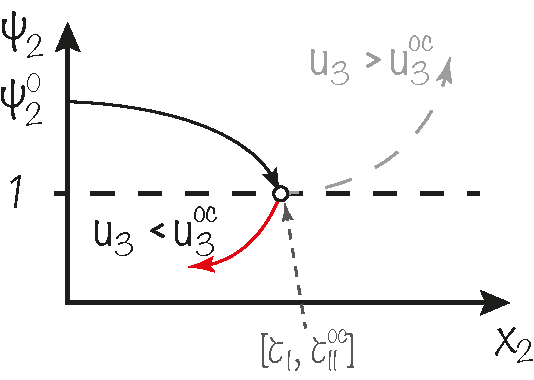
\includegraphics[height=.3\linewidth]{pic_3_4.pdf}
\end{figure}

\section*{2.1.4 Движение при $t > \tau_{II}^{\text{ос}}$}
На этом участке, как показано ранее, $u_3 ^* = 0$, следовательно, система выглядит следующим образом:
$$
    \left\{
    \begin{aligned}
        & \dot{x}_2 = - (u_1^{min} + u_2^{min} x_2) x_2, \\
        & \dot{\psi}_2 = - \psi_1 + \psi_2 (u_1^{min} + 2 u_2^{min} x_2). \\
    \end{aligned}
    \right.
$$
Начальные условия для этого участка движения выглядят следующим образом:
$$
    \left\{
        \begin{aligned}
            & x_2(\tau_I) = x_2(\tau_{II}^{\text{ос}}) = \xi, \\
            & \psi_2(\tau_{II}^{\text{ос}}) = 1.
        \end{aligned}
    \right.
$$
% TODO: начальные условия для предыдущих участков

Решение указанной задачи Коши определяет движение системы в первом квадранте $\psi_2 > 0$, $x_2 > 0$.

Возможно ли дальнейшее переключение?

\subsection*{a) переключение по $x_2$}
% TODO: картинка
Пусть $\exists \tau > \tau_{II}^{\text{ос}} \colon x_2(\tau) = 0$. Тогда, решая в обратном времени систему
$$
    \left\{
        \begin{aligned}
            & \dot{x}_2 = - (u_1^{min} + u_2^{min} x_2) x_2, \\
            & x_2(\tau) = 0,
        \end{aligned}
    \right.
$$
получим (в силу единственности решения задачи Коши) единственную траекторию $x \equiv 0$, что противоречит $x_2(\tau_{II}^{\text{ос}})$.

\subsection*{б) переключение по $\psi_2$}
Пусть $\exists \tau_{III} \colon \psi_2(\tau_{III}) = 0$. При этом имеет место параметризация $\tau_{III} = \tau_{III}(\tau_{I}, \Delta \tau_{\text{ос}})$ (время второго переключения однозначно определяется в силу единственности решения задачи Коши), то есть $\tau_{III}$ не является новым параметром.

В случае, если $\psi_2 \neq 0 \forall t \in [0, T)$, то можно положить $\tau_{III} = T$.

После указанного переключения начнёт работать $u_3^* = 0$. А что происходит с $u_1, u_2$?

Проверяем на особый режим. Пусть он возможен, тогда на протяжении некоторого времени 
$$
    0 = \dot{\psi}_2 = - \psi_1^0 + \psi_2 (u_1 + 2 u_2 x_2) = -\psi_1^0.
$$
Но по условию \eqref{eq:nonlin_3_1} из первого переключения
$$
    \psi_1^0 = u_1^{min} + 2 u_2^{min} x_2 (\tau_{I}) > 0,
$$
то есть особого режима нет.

Убедимся, что невозможен случай, когда траектория коснётся горизонтальной оси, а после вернётся обратно. В окрестности $\psi_2 = 0$:
$$
    \dot{\psi_2} = - \psi_1^0 + \psi_2 (u_1 + 2 u_2 x_2) < 0,
$$
поскольку в достаточно малой окрестности первое слагаемое отрицательно, а второе приблизительно равно нулю.

\begin{figure}[H]
    \centering
    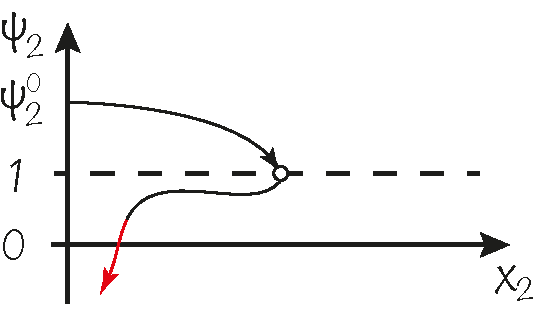
\includegraphics[height=.25\linewidth]{pic_3_5.pdf}
\end{figure}

Таким образом, после попадания в $\psi_2 = 0$ траектория системы будет направлена вниз, и произойдёт простое переключение по всем компонентам управления: при $t > \tau_{III}$
$$
\left\{
    \begin{aligned}
        & u_1^* = u_1^{max}, \\
        & u_2^* = u_2^{max}, \\
        & u_3^* = 0,
    \end{aligned}
\right.
$$
то есть начнётся фаза активного торможения.

При этом система приобретёт следующий вид:
$$
    \left\{
        \begin{aligned}
            & \dot{x}_2 = - (u_1^{max} + u_2^{max} x_2) x_2, \\
            & \dot{\psi}_2 = - \psi_1^0 + \psi_2 (u_1^{max} + 2 u_2^{max} x_2).
        \end{aligned}
    \right.
$$

\section*{2.1.5 Перебор}
Таким образом, для каждого рассматриваемого участка движения системы удалось выписать задачу Коши, однозначно определяющую её поведение. Кроме того, в ходе перепараметризации был произведён переход к паре параметров $\tau_{I}$ и $\Delta \tau_{\text{ос}}$. Осталось подобрать такие значения этих параметров, чтобы выполнялось условие на правом конце $x_1(T) = L$, $x_2(T) = \varepsilon$. Покажем, что значения обеих фазовых координат в конечный момент выражаются через введённые параметры:
$$
    \begin{aligned}
        & x_2 [T] = x_2(T, \tau_{I}, \Delta \tau_{\text{ос}}), \\
        & x_1 [T] = \int\limits_0^T x_2[t] dt = \int\limits_0^T x_2(t, \tau_{I}, \Delta \tau_{\text{ос}}) = x_1(T, \tau_{I}, \Delta \tau_{\text{ос}}).
    \end{aligned}
$$

Таким образом, для отыскания решения задачи необходимо найти все решения (относительно пары $\tau_{I}, \Delta \tau_{\text{ос}}$) системы
$$
\left\{
    \begin{aligned}
        & x_1(T, \tau_{I}, \Delta \tau_{\text{ос}}) = L, \\
        & x_2(T, \tau_{I}, \Delta \tau_{\text{ос}}) = \varepsilon,
    \end{aligned}
\right.
$$
после чего найти среди них те, которые доставляют минимально значение функционалу
$$
    J' = \int\limits_0^T u_3(t) dt = u_3^{max} \tau_{I} + u_3^{\text{ос}} \Delta\tau_{\text{ос}} + 0 \cdot (T - \tau_{I} - \Delta\tau_{\text{ос}}) = u_3^{max} \tau_{I} + u_3^{\text{ос}} \Delta\tau_{\text{ос}} \to \min.
$$

Каким образом искать решения указанной системы?

\begin{figure}[H]
    \centering
    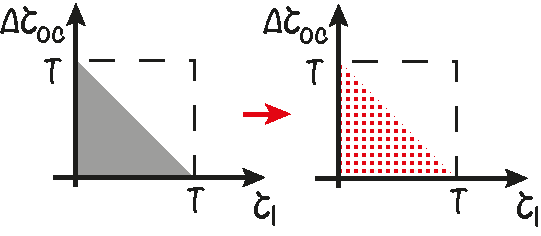
\includegraphics[height=.2\linewidth]{pic_3_6.pdf}
\end{figure}

Введём равномерную сетку \textit{(в некоторых задачах бывает удобнее работать с иной сеткой)}, зафиксируем некоторые значения $\eta > 0$ --- погрешность полученного решения, $\delta > 0$ --- шаг дискретизации параметров.

Тогда
$$
    \begin{aligned}
        & \tau_{I}^{j} = j \delta, \; j = 0, 1, \ldots, \\
        & \Delta\tau_{\text{ос}}^{i} = i \delta, \; i = 0, 1, \ldots,
    \end{aligned}
$$
при этом $(i, j) \colon \Delta \tau^i_{\text{ос}} \leqslant T - \tau_{I}^j$.

\begin{remark}
    Вообще говоря, часто $\delta = \delta(\eta)$, под каждое допустимое значение погрешности обычно подбирают соответствующий шаг сетки, однако иногда можно и просто задать оба значения.
\end{remark}

Далее осуществляется перебор всех указанных значений $(i, j)$ таких, что
$$
    \left\{
        \begin{aligned}
            & \abs{x_1(T; \tau_{I}^{j}, \Delta\tau_{\text{ос}}^{i}) - L} \leqslant \eta , \\
            & \abs{x_2(T; \tau_{I}^{j}, \Delta\tau_{\text{ос}}^{i}) - \varepsilon} \leqslant \eta.
        \end{aligned}
    \right.
$$

\begin{remark}
    Множество таких пар $(i, j)$ может быть пусто, если задача неразрешима в текущих предположениях (у нас это $\psi_1^0 > 1$) либо если шаг дискретизации $\delta$ выбран недостаточно маленьким.
\end{remark}

Наконец, как обсуждалось ранее, среди всех найденных претендентов на оптимум отбираем того, который доставляет минимум рассматриваемому функционалу.

\section*{2.1.6 Случай без особого режима в $\tau_{I}$}
Возвращаемся обратно к моменту времени $t = \tau_{I}$. Система параметризована через $(\psi_1^0, \tau_{I})$, при этом $\psi_2(\tau_I) = 1$.

Движение на участке $t > \tau_{I}$ определяется следующей системой (управление $u_3$ пока что ничего не известно):
$$
    \left\{
        \begin{aligned}
            & \dot{x}_2 = u_3 - (u_1^{min} + u_2^{min} x_2) x_2, \\
            & \dot{\psi}_2 = -\psi_1^0 + \psi_2 (u_1^{min} + 2 u_2^{min} x_2), \\
            & x_2(\tau_{I}) = \xi_2, \\
            & \psi_2 (\tau_{I}) = 1.
        \end{aligned}
    \right.
$$

Поскольку особого режима нет, то $\psi_1^0 \neq u_1^{min} + 2 u_2^{min} x_2(\tau_{I})$. Тогда, по непрерывности $\psi_2$,
$$
    \dot{\psi}_2(\tau_{I}) = - \psi_1^0 + 1 \cdot (u_1^{min} + 2 u_2^{min} x_2) < 0,
$$
что означает, что происходит простое переключение: $u_3^* = 0$ при $t > \tau_{I}$. Тогда итоговая система дифференциальных уравнений в координатах $(x_2, \psi_2)$ имеет следующий вид:
$$
    \left\{
        \begin{aligned}
            & \dot{x}_2 = - (u_1^{min} + u_2^{min} x_2) x_2, \\
            & \dot{\psi}_2 = -\psi_1^0 + \psi_2 (u_1^{min} + 2 u_2^{min} x_2), \\
            & x_2(\tau_{I}) = \xi_2, \\
            & \psi_2 (\tau_{I}) = 1.
        \end{aligned}
    \right.
$$

По аналогии с предыдущими рассуждениями можно показать, что $x_2 > 0$.

Следовательно, характер движения системы может измениться только при наступлении $\psi_2(\tau_{II}) = 0$.

\begin{figure}[H]
    \centering
    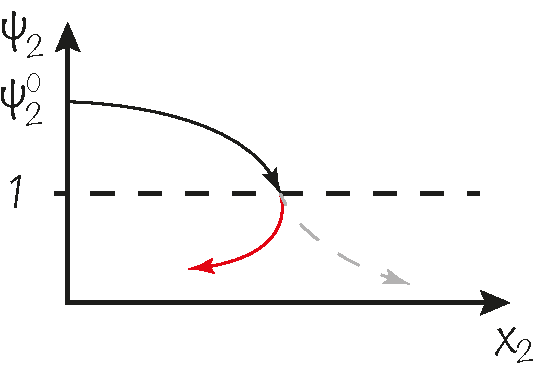
\includegraphics[height=.3\linewidth]{pic_3_7.pdf}
\end{figure}

\subsection*{а) Особый режим?}
Возможен ли при этом особый режим? Ранее он не был возможен в силу ограничения на значение $\psi_1^0$, теперь же такого ограничения нет, и
$$
    0 = -\psi_1^0 + 0 \cdot (u_1^{min} + 2 u_2^{min} x_2) \thus \psi-1^0 = 0.
$$
Однако последнее условие противоречит ходу решения. Действительно, проинтегрируем систему в обратном времени при $t < \tau_{II}$:
$$
    \left\{
        \begin{aligned}
            & \dot{\psi}_2 = \psi_2 (u_1^{min} + 2 u_2^{min} x_2) = \psi_2 \tilde{\alpha}(t), \\
            & \psi_2 (\tau_{II}) = 0.
        \end{aligned}
    \right.
    \thus \psi_2(t) = \mathbf{e}^{\int\limits_{\tau_{II}}^t \tilde{\alpha}(s) ds} \cdot \psi_2 (\tau_{II}) \equiv 0,
$$
что приводит нас к противоречию ($\psi_2(\tau_{II}-0) > 0$).

\subsection*{б) Простое переключение}
Таким образом, особого режима в этом случае нет, и имеет место ещё одно простое переключение: $u_3^* = 0$, $u_1^* = u_1^{max}$, $u_2^* = u_2^{max}$ при $t > \tau_{II}$, и
$$
    \left\{
        \begin{aligned}
            & \dot{x}_2 = - (u_1^{max} + u_2^{max} x_2) x_2, \\
            & \dot{\psi}_2 = -\psi_1^0 + \psi_2 (u_1^{max} + 2 u_2^{max} x_2), \\
            & x_2(\tau_{I}) = \xi_2, \\
            & \psi_2 (\tau_{I}) = 1.
        \end{aligned}
    \right.
$$

\subsection*{Перепараметризация}
Выразим $\psi_1^0 = \psi_1^0(\tau_{I}, \tau_{II})$, чтобы снова перейти к более удобным параметрам. Как произвести такую перепараметризацию?

\begin{enumerate}
    \item Получаем траекторию $x_2(t)$ при $t \in [\tau_{I}, \tau_{II}]$:
    $$
        \frac{dx_2}{x_2(u_1^{min} + u_2^{min} x_2)} = -dt,
    $$
    раскладываем на простые дроби и получаем $x_2(t; \tau_I, \tau_{II})$.
    \item Формально проинтегрируем дифференциальное уравнение на $\psi_2$:
    $$
        0 = \psi_2(\tau_{II}) = \psi_2(\tau_{I}) \cdot \mathbf{e}^{\int\limits_{\tau_I}^{\tau_{II}} \tilde{\alpha}(s) ds} + (-\psi_1^0) \cdot \int\limits_{\tau_{I}}^{\tau_{II}} \mathbf{e}^{\int\limits_{t}^{\tau_{II}} \tilde{\alpha}(s) ds} dt.
    $$
    Подставляя $\psi_2(\tau_I) = 1$, выразим $\psi_1^0$ через $\tau_I$ и $\tau_{II}$.
\end{enumerate}

Таким образом, перешли к параметрам $(\tau_{I}, \tau_{II})$, где $0 \leqslant \tau_{I} \leqslant \tau_{II} \leqslant T$. Как и ранее, если $\tau_{I} > T$, положим $\tau_{I} = T$, если $\tau_{II} > T$, положим $\tau_{II} = T$.

\begin{figure}[H]
    \centering
    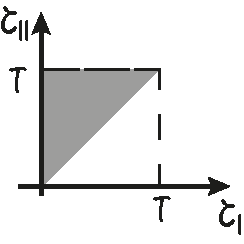
\includegraphics[height=.2\linewidth]{pic_3_8.pdf}
\end{figure}

Сопряжённые переменные при этом нужны только для построения, это некоторая вспомогательная конструкция, через которую удобно выразить $u$ в начале решения, однако конечный перебор чаще всего удобнее осуществлять по другим параметрам.

Перебирая значения параметров, необходимо решить систему:
$$
    \left\{
        \begin{aligned}
            & x_1[T] = L, \\
            & x_2[T] = \varepsilon > 0.
        \end{aligned}
    \right.
$$

В данном случае возможно понизить размерность перебора. Вспомним, в силу каких дифференциальных уравнений двигается система на различных отрезках времени:
\begin{enumerate}
    \item[(I)] $\dot{x}_2 = u_3^{max} - (u_1^{min} + u_2^{min} x_2) x_2, \qquad t \leqslant \tau_{I}$;
    \item[(II)] $\dot{x}_2 = - (u_1^{min} + u_2^{min} x_2) x_2, \qquad t \in (\tau_I; \tau_{II}]$;
    \item[(III)] $\dot{x}_2 = - (u_1^{max} + u_2^{max} x_2) x_2, \qquad t > \tau_{II}$. 
\end{enumerate}

Выразим $\tau_{II}$ через $\tau_{I}$:
\begin{itemize}
    \item из (I) и $x_2(0) = 0$ $\thus$ $x_2(\tau_{I}) = \xi_2$;
    \item из (II) и $x_2(\tau_{I}) = \xi_2$ $\thus$ $x_2(\tau_{II}) = x_2^{\text{лев}}(\tau_{II}; \tau_{I}, \xi_2)$;
    \item из (III) и $x_2(T) = \varepsilon$ $\thus$ $x_2(\tau_{II}) = x_2^{\text{прав}}(\tau_{II}; T, \varepsilon)$.
\end{itemize}
Из уравнения
$$
    x_2^{\text{лев}}(\tau_{II}; \tau_{I}, \xi_2) = x_2^{\text{прав}}(\tau_{II}; T, \varepsilon)
$$
находим выражение $\tau_{II} = \tau_{II}(\tau_{I}, T, \varepsilon)$. Это соотношение задаёт выражение одного параметра через другой, таким образом, позволяя опустить перебор по $\tau_{II}$.

\begin{figure}[H]
    \centering
    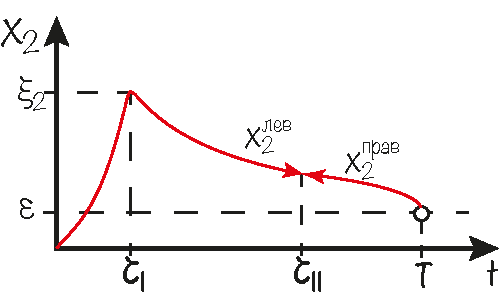
\includegraphics[height=.3\linewidth]{pic_3_9.pdf}
\end{figure}

Исключив таким образом параметр $\tau_{II}$, можем понизить размерность сетки для перебора, получив однопараметрическое семейство траекторий, зависящих от $\tau_{I}$. При этом, ввиду произведённых манипуляций, вместо системы на $(x_1[T], x_2[T])$ необходимо будет проверить только уравнение $x_1[T] = L$ \textit{(второе уравнение мы напрямую <<встроили>> в решение)}.

\section*{Шаг 2.2 Движение при $\psi_2^0 < 1$}

Выпишем систему ОДУ, в силу которой будет двигаться наша тележка: поскольку в силу (УМ) $u_3^*(0+) = 0$,
$$
    \left\{
    \begin{aligned}
        & \dot{x}_1 = x_2, \\
        & \dot{x}_2 = - (u_1 + u_2 x_2) x_2, \\
        & \dot{\psi}_1 = 0, \\
        & \dot{\psi}_2 = - \psi_1^0 + \psi_2 (u_1 + 2 u_2 x_2), \\
        & \dot{x}_2(0) = 0, \\
        & u_1^* = ?, \; u_2^* = ?
    \end{aligned}
    \right.
$$

В силу единственности, для этой системы $x_2 \equiv 0$ --- единственное решение. Таким образом, движение начнётся только в тот момент $\tau_{\text{нач}}$, когда включится условие $u_3 >0$, то есть будет $\psi_2 \geqslant 1$:
$$
    \psi_2(\tau_{\text{нач}}) = 1, \; \psi_2(t) > 1 \text{ при } t \in (\tau_{\text{нач}}, \tau_{\text{нач}} + \delta) \text{ по непрерывности },
$$
то есть $u_3^* = u_1^{max}$ при $t > \tau_{\text{нач}}$. В этот момент произойдёт переключение по остальным компонентам управления, и начнётся движение:
$$
    u_1^* = U_1^{max}, \; u_2^* = u_2^{min} \text{ при } t > \tau_{\text{нач}}.
$$

\begin{figure}[H]
    \centering
    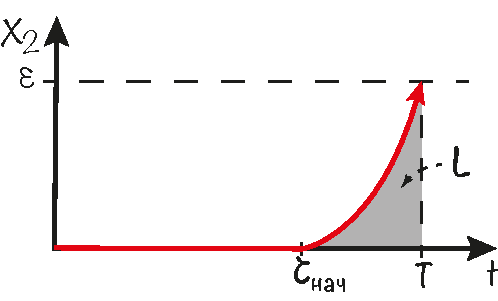
\includegraphics[height=.25\linewidth]{pic_3_10.pdf}
\end{figure}

Здесь мы вспоминаем про условие из самого начала постановки задачи:
$$
    L > T\varepsilon.
$$
Здесь же площадь криволинейной трапеции под графиком выше меньше площади прямоугольника, обозначенного пунктиром:
$$
    L = \int\limits_0^T x_2(\tau) d\tau \leqslant \varepsilon (T - \tau_{\text{нач}}) < T\varepsilon.
$$

Таким образом, этот случай невозможен.

\section*{Шаг 2.3 Движение при $\psi_2^0 = 1$}
Данный случай полностью повторяет предыдущий пункт, однако теперь возможен вариант $\tau_{\text{нач}} = 0$. Так или иначе, условие $L > T \varepsilon$ всё ещё делает этот случай невозможным \textit{(был бы возможен при ограничении $L \geqslant T \varepsilon$)}.

\section*{Шаг 3. Анормальный случай}
$$
    \psi_0 = 0
$$

В чём отличие от нормального случая? В условиях на $u_3^*$:
$$
    u_3^* = 
        \left\{ 
            \begin{aligned}
                & u_3^{max}, &\psi_2 > 0, \\
                & [0, u_3^{max}], &\psi_2 = 0, \\
                & 0, &\psi_2 < 0.
            \end{aligned} 
        \right.
$$
Остальные компоненты управления остаются такими же:
$$
u_1^* = \left\{ \begin{aligned}
    & u_1^{min}, &\psi_2 x_2 > 0, \\
    & [u_1^{min}, u_1^{max}], &\psi_2 x_2 = 0, \\
    & u_1^{max}, &\psi_2 x_2 < 0,
\end{aligned} \right.
\qquad
u_2^* = \left\{ \begin{aligned}
    & u_2^{min}, &\psi_2 > 0, x_2 \neq 0, \\
    & [u_2^{min}, u_2^{max}], &\psi_2 x_2 = 0, \\
    & u_2^{max}, &\psi_2 < 0, x_2 \neq 0,
\end{aligned} \right.
$$

Движение будет происходить по аналогии с нормальным случаем.

Пусть $\psi_2^0 > 0$. Возможен ли особый режим при переходе через $\psi_2 = 0$? Пусть да, тогда
$$
    0 = \dot{\psi}_2 = -\psi_1^0 + 0 \cdot (\ldots) \thus \psi_1^0 = 0 \thus (\psi_0, \psi_1, \psi_2) = 0
$$
на отрезке времени ненулевой меры, что противоречит (УН). То есть особый режим не возможен, происходит простое переключение по всем трём компонентам управления.

Перепараметризуем, переходим к параметру $\tau_I \colon \psi_2(\tau_I) = 0$. Поскольку при этом $\psi(\tau_I) \neq 0$, то $\psi_1(\tau_I) \neq 0$. Поскольку мы нормируем в начальный момент времени: $\psi_1(\tau_I) = \psi_1^0 = 1$ (случай $\psi_1^0 = -1$ исключаем, т.к. по доказанному ранее это влечёт $\psi_2 \uparrow$, и мы никогда не затормозим).

Таким образом, зафиксировав $\psi_0^0, \psi_1^0$ и перейдя к перебору по $\tau_I$, получаем однопараметрическое семейство решений.

\begin{remark}
    Анормальный случай --- предельный для нормального при $\tau_I = \tau_{II}$.
\end{remark}

\begin{exercise}
    Рассмотреть эту систему при 
    $$
        u_3 \in [u_3^{min}, u_3^{max}], \qquad J = \int\limits_0^T \abs{u_3(t)} dt,
    $$
    где $u_3^{min} < 0 < u_3^{max}$.
\end{exercise}